% !TeX root = ../dissertation.tex

\begin{figure*}[!th]
	\centering
	\begin{subfigure}{.6\columnwidth}
		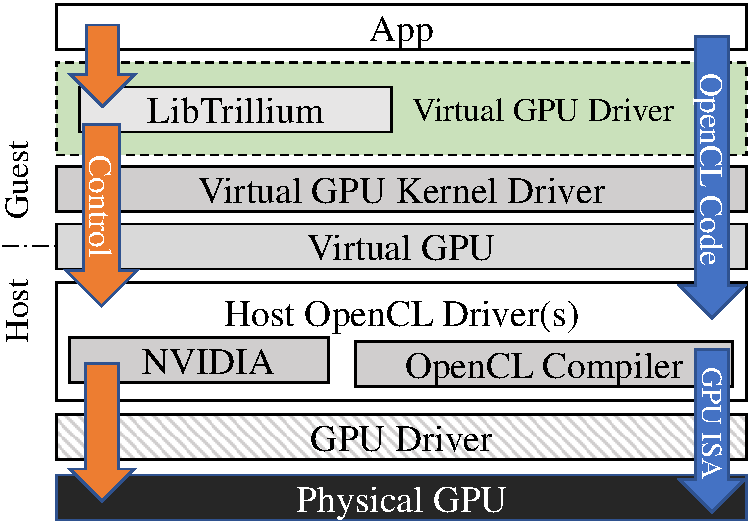
\includegraphics[width=\columnwidth,trim={0cm 0cm 0cm 0cm},clip]{trillium/images/design/trillium_design.pdf}
		\caption{{}}
		\label{fig_trillium}
	\end{subfigure}\hfill
	\begin{subfigure}{.72\columnwidth}
		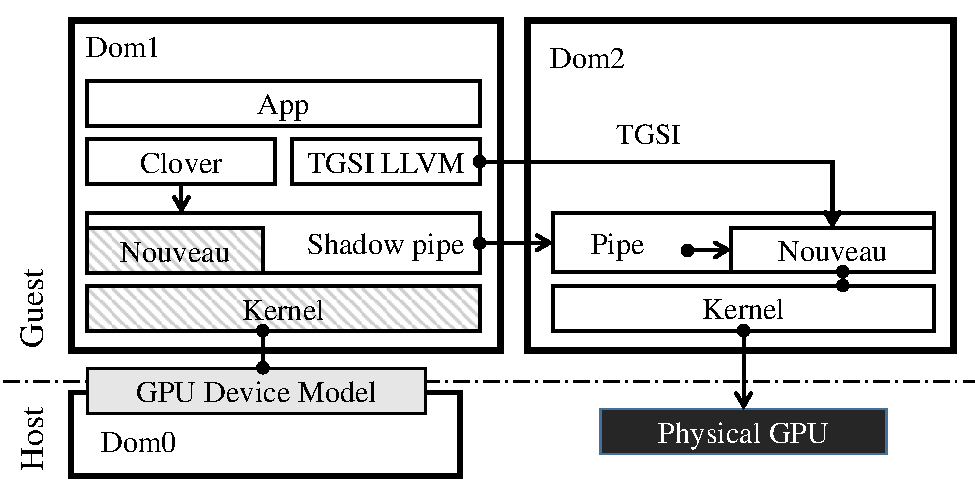
\includegraphics[width=\columnwidth,trim={0 0 0 0},clip]{trillium/images/design/xen-svga.pdf}
		\caption{{}}
		\label{fig_trillium_classic}
	\end{subfigure}\hfill
	\begin{subfigure}{.68\columnwidth}
		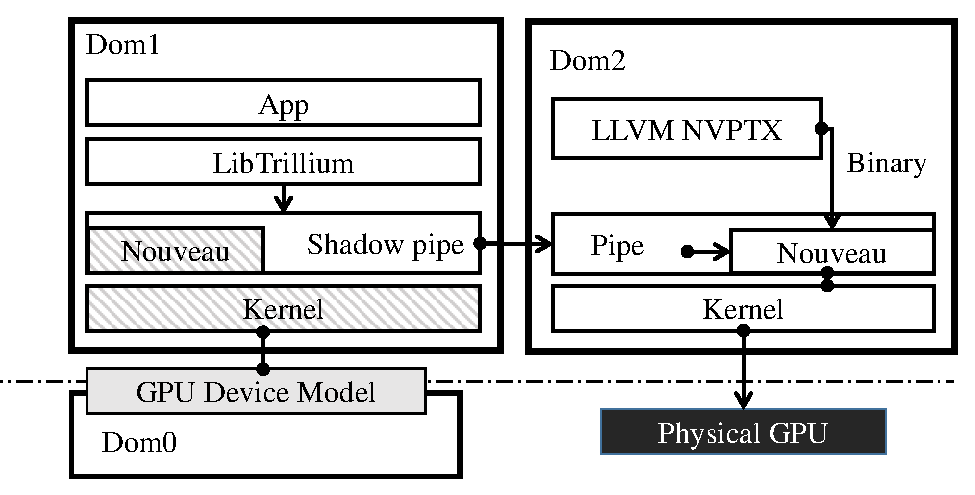
\includegraphics[width=\columnwidth,trim={0.6cm 0 0 0},clip]{trillium/images/design/trillium.pdf}
		\caption{{}}
		\label{fig_trillium_direct}
	\end{subfigure}
	\caption{{\footnotesize \trxc and \Trillium designs. (a) The \Trillium stack. (b) \trxc approximates the SVGA model extended to support GPU Compute. (c) The design of \trillium with shadow pipe.}}
	% \hyu{I'd like to unify the styles(colors)}
\end{figure*}

\section{Implementation}
\label{sec_implementation}

We evaluated the \Trillium design against a representative of each traditional virtualization
technique: full-virtualization, user-space API-remoting and SVGA.
% interposition mechanism
% in order to empirically measure the trade-offs posed by each of the myriad
% designs proposed in the literature.
Due to the difficulty of implementing a trap-based virtualization scheme,
we chose to evaluate against GPUvm~\cite{GPUvm},
the only existing open-source implementation.
%~\footnote{https://github.com/CPFL/gxen/}.
GPUvm is tightly coupled with the Xen hypervisor~\cite{barham2003xen}.
As a result, all the other prototypes were built on the Xen hypervisor
to keep the platform common for fair comparison.

\begin{figure}[!th]
	\centering
	\begin{subfigure}{.45\columnwidth}
		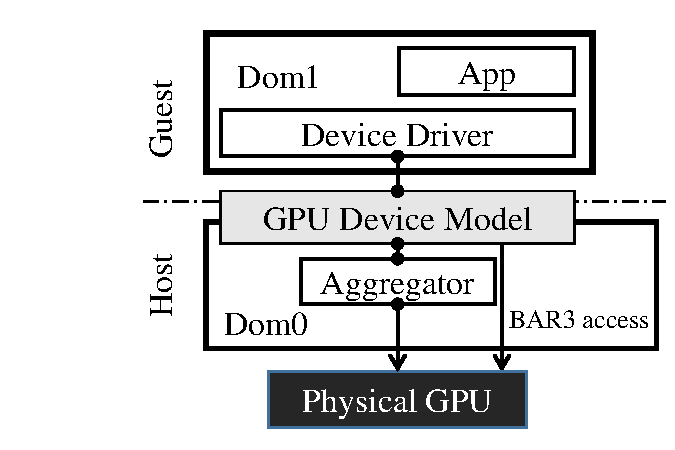
\includegraphics[width=\columnwidth,trim={2cm 0cm 0cm 0cm},clip]{trillium/images/design/gpuvm.pdf}
		\caption{{}}
		\label{fig_gpuvm_basic}
	\end{subfigure}\hfill
	\begin{subfigure}{.55\columnwidth}
		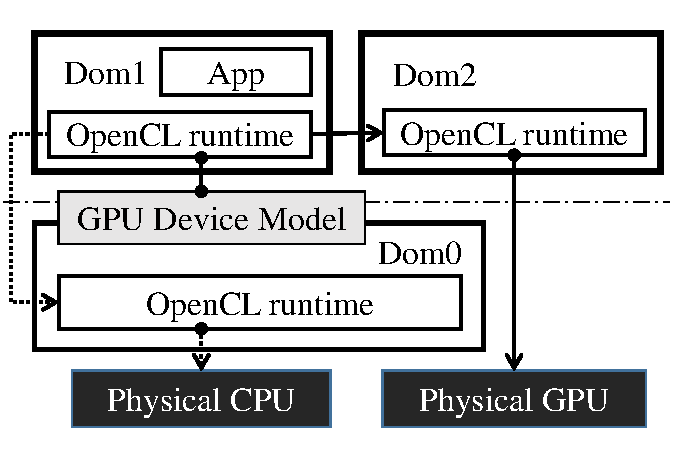
\includegraphics[width=\columnwidth,trim={0 0 0 0},clip]{trillium/images/design/api-remote.pdf}
		\caption{{}}
		\label{fig:api_remote}
	\end{subfigure}
	\caption{{\footnotesize Xen-based virtualizaton designs. (a) Trap-based virtualization: GPUvm. (b) User-space API remoting over RPC---dashed arrows indicate \apicpu, while solid ones indicate \apigpu.}}
\end{figure}

\subsection{Trillium}

%Although the \Trillium design is envisioned, and presented as an extension
%to the VMware ESX virtualization stack in Section~\ref{sec:trillium_design} and Figure~\ref{fig_trillium}, the same
%techniques are implemented
%We implement Trillium on the Xen platform.


%\begin{figure}[!th]
%	\centering
%	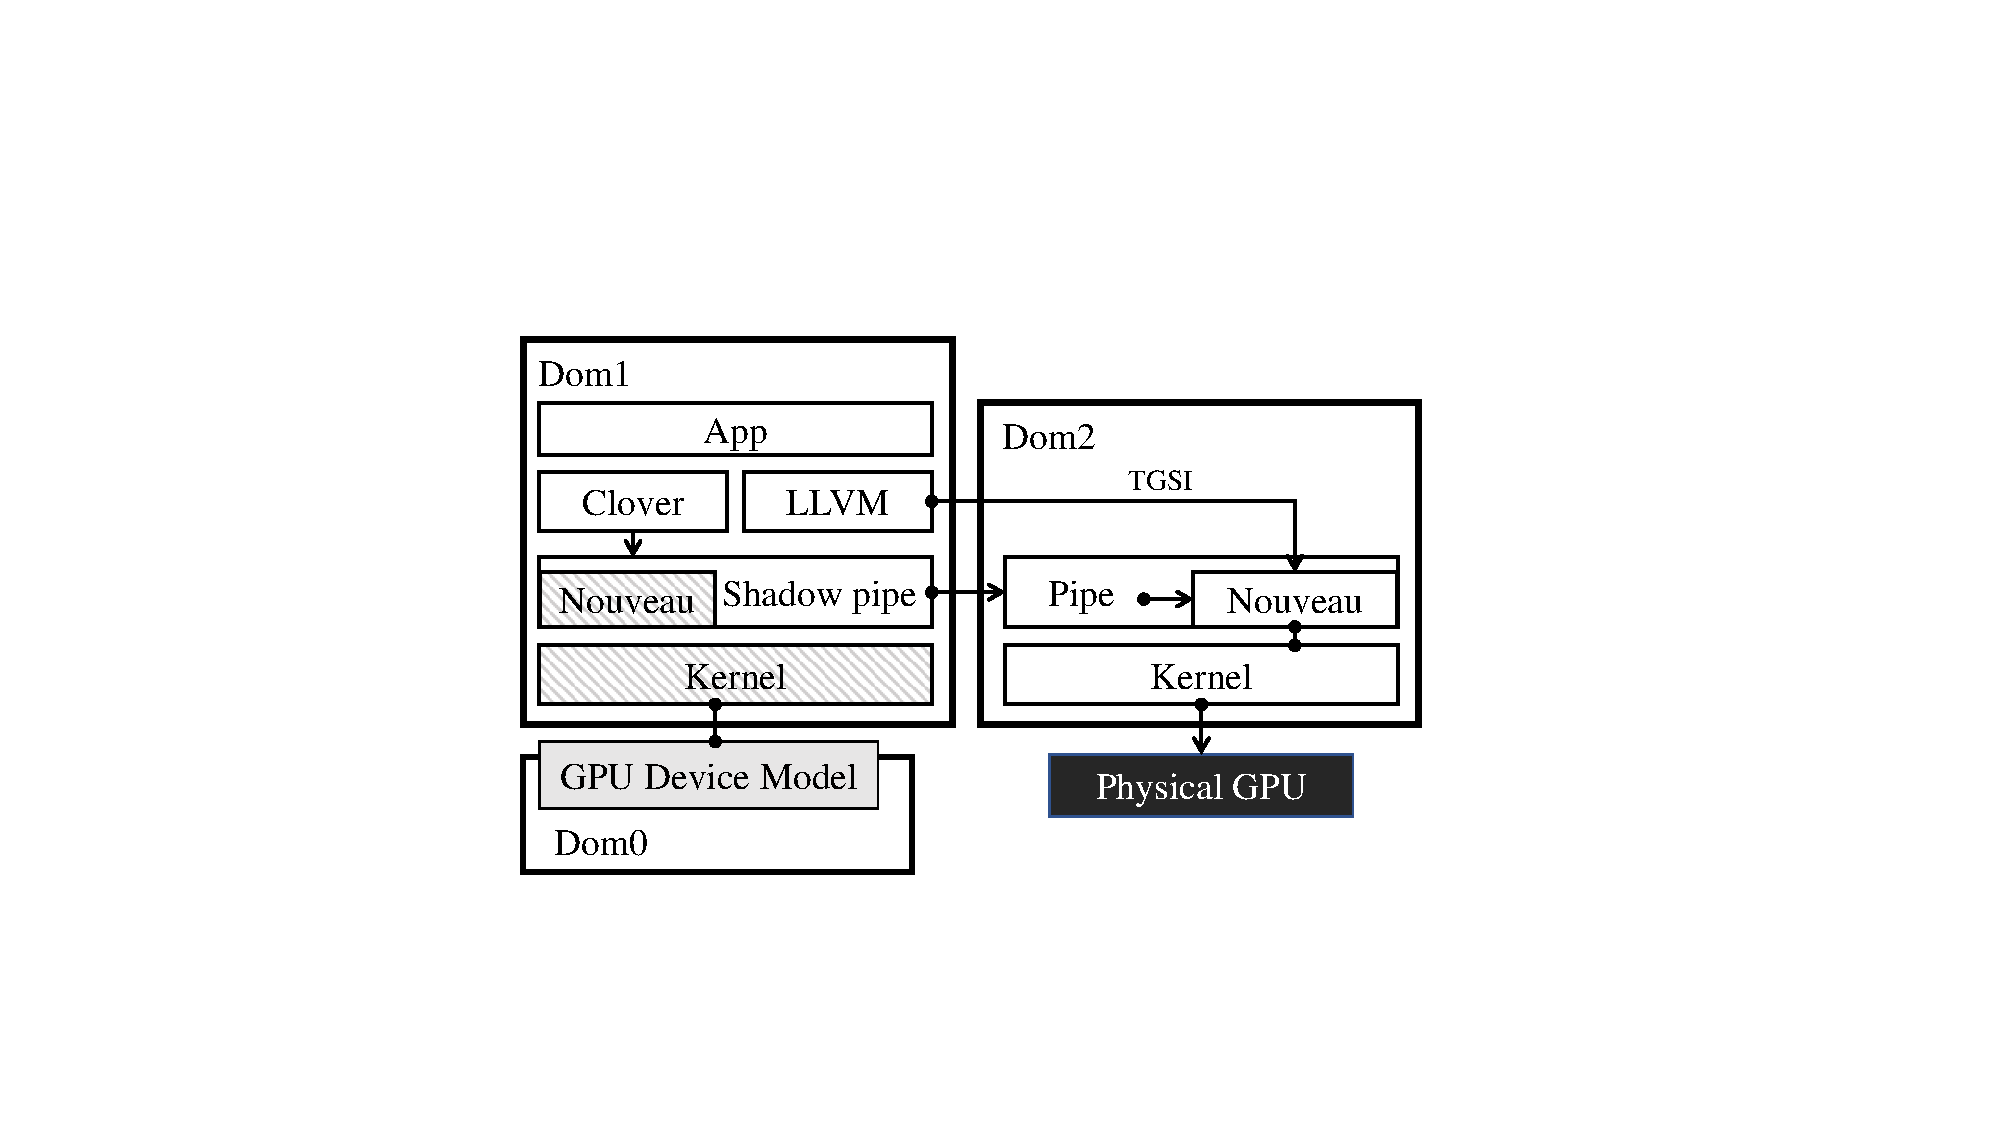
\includegraphics[width=.9\linewidth,trim={8cm 4cm 8cm 5.5cm},clip]{images/trillium/trillium_classic.pdf}
%	\caption{{\footnotesize \trxc approximates the SVGA model extended to support GPU Compute.
%            \cjr{FIXME: get designs in position as discussed with Hangchen. }}}
%	\label{fig_trillium_classic} \end{figure}
%
%\begin{figure}[!th]
%	\centering
%	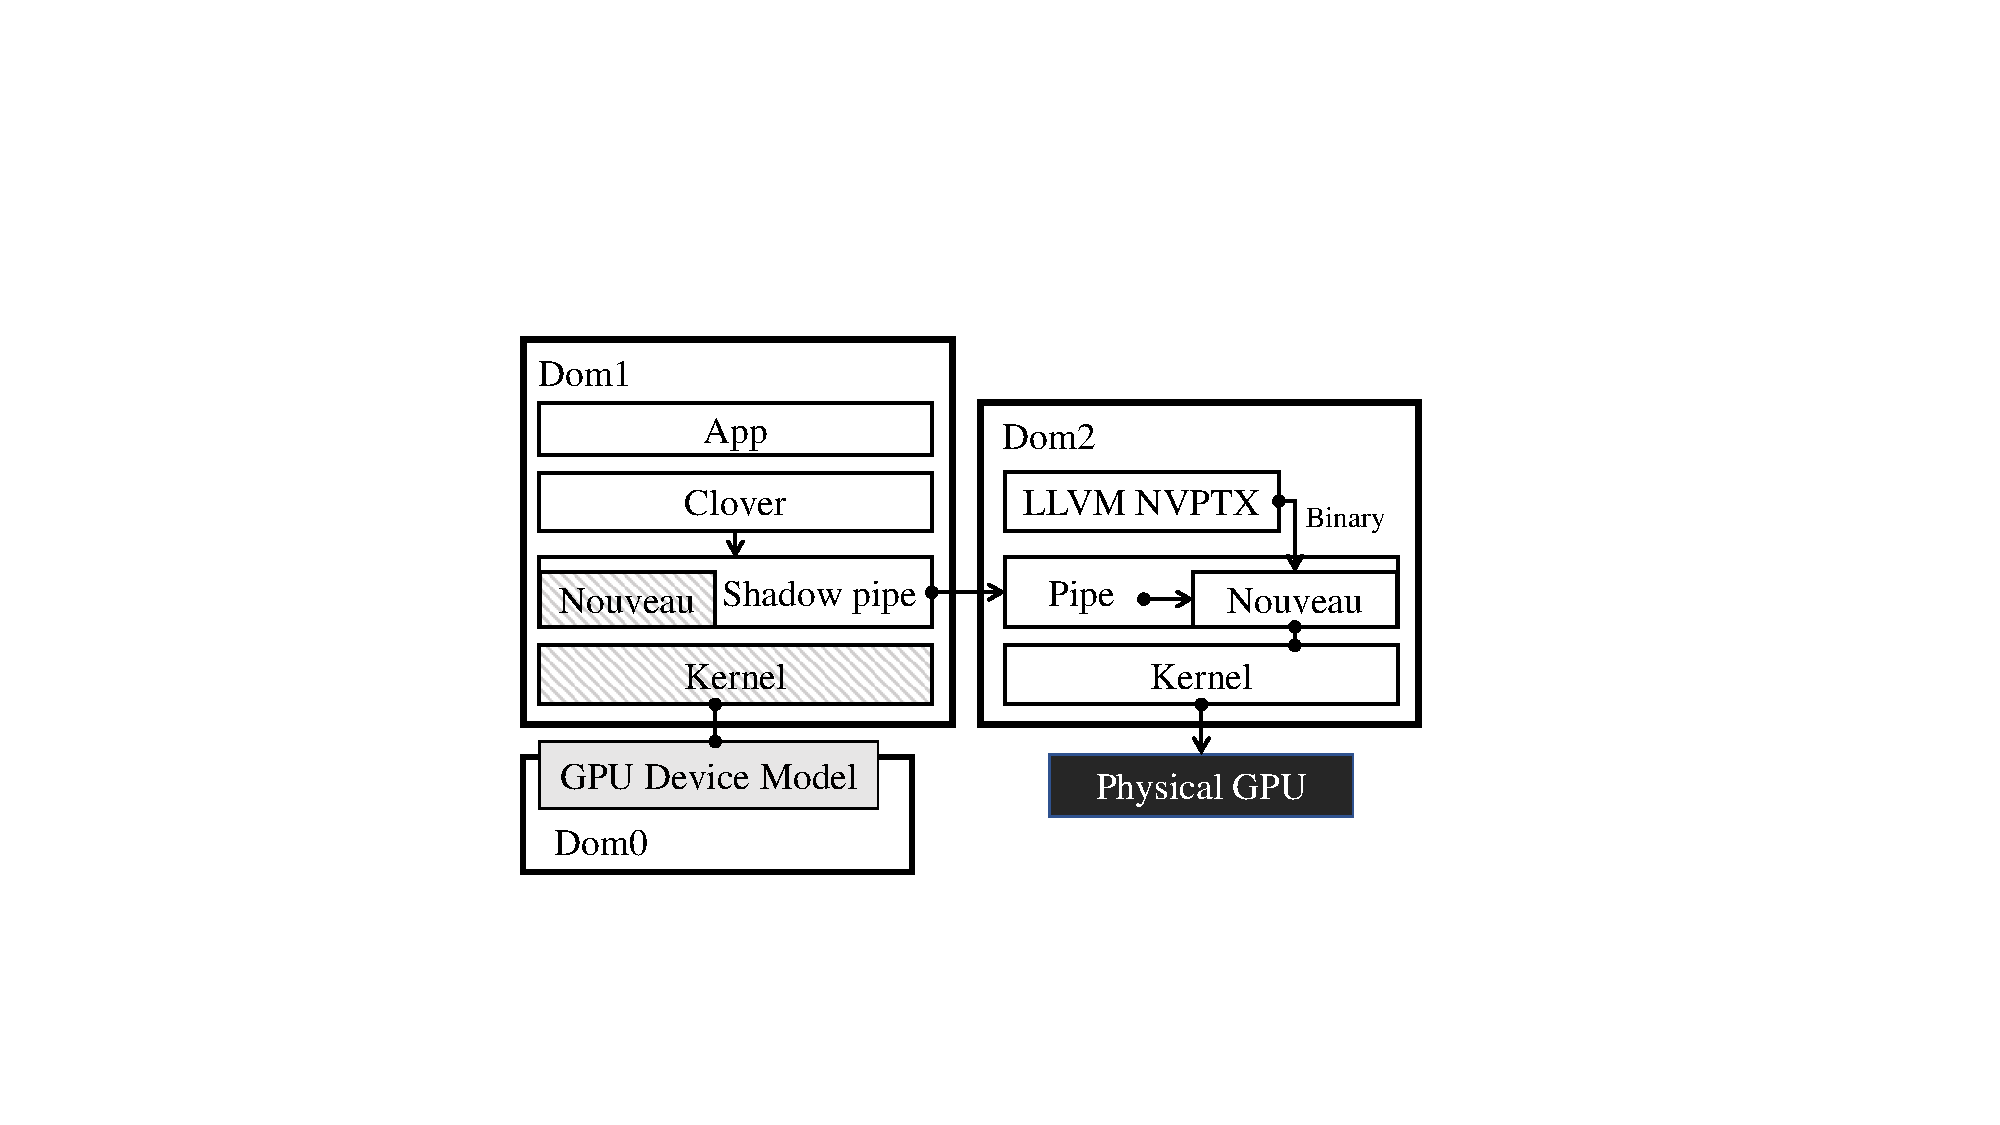
\includegraphics[width=.9\linewidth,trim={8cm 4cm 8cm 5.5cm},clip]{images/trillium/trillium_direct.pdf}
%	\caption{{\footnotesize The design of Trillium Direct with shadow pipe.
%            \cjr{FIXME: get designs in position as discussed with Hangchen. }}}
%	\label{fig_trillium_direct} \end{figure}

We initially implemented \Trillium on Xen following the SVGA
design, by implementing OpenCL support in a virtual device and extending
the Mesa stack with TGSI support (see Section~\ref{ssec:tgsi_backend}
for details). The generated TGSI is sent to the host via RPC, and then
finalized to a binary that can be run on the physical NVIDIA GPU using
the open source Nouveau driver.
Upon empirically finding that TGSI is a performance bottleneck, we revisited
the basic design. We preserve the original prototype, hereafter called \trxc,
as a baseline representative of the original SVGA design:
this design is shown in Figure~\ref{fig_trillium_classic}.
The current \Trillium design is shown in Figure~\ref{fig_trillium_direct}.

\trxc and \trxd, implement API-forwarding in a custom pipe-driver in Gallium3D,
that we call \shadowpipe. We chose to forward the pipe-driver as it is presents a
narrow interposition interface in the graphics driver. However, given that each OpenCL
API call is decomposed into many different pipe-driver calls,
% there may be
other APIs higher up in the graphics stack may be better suited for interposition.
% Our choice of implementing interposition using \shadowpipe should be
% considered an implementation detail, and not prescriptive in the \Trillium
% design.
The \shadowpipe is in the \textit{application domain}'s graphics
stack, and shims the pipe-driver interface as RPC calls to the actual Nouveau
pipe-driver in the \textit{privileged domain}.

\trxc manages user-level contexts, command queues and memory objects; and
translates the input OpenCL GPGPU kernel to TGSI in the application domain.
% using the back-end TGSI compiler.
\trxd skips the compilation phase in the application domain.
The OpenCL kernel is forwarded to the privileged domain
via RPC, where it is parsed and compiled by the LLVM NVPTX back-end in
parallel. This binary is then loaded onto the GPU when the pipe-driver hits
the binary loading phase.
\Trillium can also
% leverage the Clover stack to
emit LLVM IR if an OpenCL compiler is not available in the host.

%\aak{Are we changing the story to say that \Trillium uses LLVM IR?}
%\cjr{We are changing to say it \emph{can} but is flexible}

% RPC introduces additional network overhead between application- and
% privileged- domains.

Our implementation relies on gRPC as a transport mechanism between the
guest and the host, as an implementation convenience. As zero-copy
transfer~\cite{chu1996zero,tezuka1998pin} and
hypercall~\cite{ram2010redesigning} mechanisms are well-studied, and
a production-ready version of \Trillium would rely on these mechanisms,
we measure and remove transport
overhead from our reported measurements in Section~\ref{sec:eval}.
The overheads stem from remoting calls to the privileged domain over the network, which is especially significant since a single
OpenCL API call may be decomposed into many pipe-driver APIs, and from
the large amount of kernel input data that must be copied between VMs.
% However, we use this primarily as an implementation convenience, as zero-copy~\cite{chu1996zero,tezuka1998pin} and hypercall~\cite{ram2010redesigning} mechanisms are well studied solutions to this problem.

\paragraphbe{LLVM TGSI Back-end}
\label{ssec:tgsi_backend}
% \cjr{Vulkan standard wants to supercede Gallium3D; replacing TGSI with SPIR-V. Maybe that would solve everything.}
The Mesa3D stack implements OpenCL support via a state-tracker called Clover.
Clover provides the library for the OpenCL application to link against, while
most of the compilation is handled by invoking the OpenCL and C++ front-ends
of the LLVM~\cite{lattner2004llvm} compiler framework. Clover provides much of
the front-end infrastructure required to support GPGPU computing in \trxc and \Trillium.
% However, LLVM lacks a working TGSI back-end.

% Clover works well for AMD GPUs thanks to contributions by AMD community.
Historically, lack of a working TGSI back-end in LLVM, despite several attempts
at building one in the past 5 years~\cite{old_llvm_tgsi1,old_llvm_tgsi2}, has
left OpenCL support for NVIDIA GPUs and SVGA in Mesa3D incomplete.
% A closed source implementation, based on the CUDA framework, is available for NVIDIA GPUs.
In order to support OpenCL in \trxc, we implemented an LLVM TGSI back-end.
While the TGSI back-end is not yet mature, we have added
support for a majority of the 32-bit integer and floating point operations,
intrinsics, memory barriers, and control flow. Using this backend we are
able to compile and run 10 out of the 12 Rodinia benchmarks~\cite{che2009rodinia}
used to benchmark GPUvm. Because the compiler is built using the LLVM framework,
it enjoys all of the IR-level optimizations in LLVM.

% To provide a meaningful baseline against which to evaluate \Trillium, we needed
% OpenCL support in Mesa, which in turn required us to implement a TGSI back-end for
% LLVM.\cjr{any interesting statistics? Man-years? SLoC? Limitations worth mentioning, like it's not super-optimized yet?}
% \aak{In total we've added 56 lines to libclc, 2079 lines to the TGSI backend, and 156 lines to Mesa. It's not super-optimized but benefits from IR level optimizations courtesy of LLVM.}

% \Trillium-classic is implemented by completing the skeletal OpenCL implementation
% in the open source Mesa~17.2 graphics stack. We implemented the missing OpenCL to TGSI
% compilation as a TGSI backend in LLVM and clang~4.0. \cjr{Amogh, any additional comments here?
% would be great to get a sense of the scale of the effort. It didn't begin with the TGSI,
% you had to first fix a bunch of adjacent parts of the runtime too, right? What required
% fixing? How many SLoC in your implementation? The TGSI implementation isn't complete
% right? Can you summarize what's still on the TODO. Should observe the obvious: it's not optimized.}.
% In addition to the substantial effort that went into implementing the TGSI back-end, we also had to
% bringing the code up to date, fixing API mismatches between the clover implementation which was a year old and the LLVM trunk, tracking down initialization bugs (number of threads).
% We've fixed the get\_thread\_id implementation in LibCLC, and added barrier and membar intrinsics.
% The TGSI implementation isn't complete, but implements a majority of the  integer, and floating point parts of the ISA. The more esoteric options like vote. Control flow was the biggest part of the TGSI implementation, although most of the code was copied over from the AMD back-end and modified to suit our needs.
% \cjr{maybe this moves to implementation.}

LLVM IR handles control flow by using conditional and unconditional
branches to and from Basic Blocks. A majority of the usual
optimizations (constant propagation, loop unrolling, etc) are applied
on the IR. On the other hand, TGSI assumes a linear control flow
through the program, using higher level constructs such as
IF-THEN-ELSE, FOR and WHILE loops. To accommodate this difference in
control flow techniques, we leveraged a similar implementation in the
AMDGPU back-end which calculates a Strongly-Connected-Components (SCC)
graph from the Basic Block-based control flow in the LLVM IR, and then
duplicates Basic Blocks as necessary. It is a testament to the
maturity and flexibility of LLVM that the infrastructure to produce an
SCC, and an example of how to use it to raise the control flow
abstraction level were readily available.
% The total implementation took only 2000 lines of code in our back-end.

\subsection{GPUvm}

GPUvm~\cite{GPUvm} is an open-source trap-based interposition design (a simplified block-diagram
representation is shown in Figure~\ref{fig_gpuvm_basic}).
% introduced in section~\ref{sec:bg_fullvirt} and\ref{sec:gpuvm},
The application domain (Dom 1) is presented with a GPU Device Model,
which is emulated in the privileged domain (Dom 0).
The emulation layer in Dom 0 interposes, validates, and fulfills
all attempts to access the GPU.
% and fulfills the requested operations after .
% is the only open source full-virtualization solution we could find, but it
GPUvm has not been maintained: The last release, in 2012, is based on Xen 4.2.0
and runs on Fedora~16~\cite{yu2017fullvirt}. In order to compare all prototypes on
the same modern platform, we ported GPUvm to Ubuntu~16.04 with Xen~4.8.2.
% Dependencies were also resolved to use the default Xenial libraries.


% \subsection{CPU-backend GPUvm}

% Previous works have evaluated the performance of GPUvm, and found significant
% overheads in its full-virtualization design~\cite{suzuki2014gpuvm,yu2017fullvirt}. As lots of
% I/O instructions are emulated by software, we should consider the power of CPU
% to execute the GPU workloads directly.

% Intel provides an OpenCL runtime driver for its CPUs. Instead of executing
% OpenCL commands in the guest, they are forwarded to the hypervisor and executed
% on CPU. A faked GPU device model is provided to the guest, fooling the guest that
% it is using a GPU hardware. The model is shown in Figure~\ref{fig_gpuvm_cpu}. The calls can be
% forwarded via either RPC or Xen bus.

% \subsubsection{Runtime API forwarding}

% To compare with the CPU-backend GPUvm and Trillium models, we also implemented
% an pure API-forwarding prototype. API calls are forwarded to an OpenCL server which
% can be the hypervisor, another VM, or a remote machine which has OpenCL runtime.
% The design is shown in Figure~\ref{fig_gpuvm_api}. The API calls is forwarded via RPC in this design.


% \subsubsection{CPU-backend GPUvm}

\subsection{User-space API remoting over RPC} \label{sec:api_remote_design}

% We also implement two user-level API remoting over RPC schemes, here-after
% referred to as \texttt{remote-gpu} and \texttt{remote-cpu}.
In order to faithfully mimic user-level API-remoting-over-RPC
systems~\cite{rCUDA,kim2012snucl,bitfusion-whitepaper},
OpenCL API calls are trapped by a user-space shim library and forwarded via RPC
from one appliance VM, which is the OpenCL ``client'',
to another appliance VM, which acts as the OpenCL ``server''.
% The OpenCL
% server can be either an appliance VM or a physical machine with
% accessible compute devices, running an efficient aggregator which
% collects, manages, and marshals data and mapped virtual objects,
% and executes remote OpenCL calls.
Figure~\ref{fig:api_remote} shows the setup of the two API-remoting schemes
we considered: \apigpu and \apicpu.
The black arrows indicate the workflow of \apigpu, where the OpenCL server
runs the OpenCL commands on a physical GPU using the NVIDIA OpenCL
framework. The grey arrows show the \apicpu setup, where the OpenCL commands
are executed on a multi-core CPU (Intel CPU Xeon E5-2643) using the Intel
OpenCL SRB~5.0 framework.
% Remoting a high-level API like OpenCL make the task of supporting various underlying hardware less daunting.
RPC is implemented using gRPC~1.6 (based on Google ProtocolBuffers~3.4.0) and
inter-service communications are implemented over XML-RPC~1.39. Lower-overhead
data-movement techniques, such as zero-copy, can be applied when both the
client and the server are on a local machine.

\subsection{Optimizations}
\label{sec:optimizations}
\trillium interposes at the pipe-driver API yielding fine-grained interposition,
and therefore finer-grained multiplexing of the GPGPU.
However, interposing at this layer also results in significant transport overhead.
Many pipe-driver functions are responsible for context management and information retrieval---%
operations that do not result in interaction with the GPU.
We reduce communication overhead by batching these types of API-calls, taking care to
fall back to synchronous API-forwarding when any pipe-driver API calls that interact
with the physical GPU are invoked.

% executing all such operations on the application
% domain, only synchronizing with the privileged domain at predefined barriers.
% We modify the benchmark applications we run on \trillium
% by inserting synchronization barriers at regular intervals, and batch the
% execution of pipe-driver API calls between synchronization points on both
% domains simultaneously.
% Occasionally execution is faster in the one of the
% domains, in which case a synchronization message with updated context
% information is issued to the other domain, which instructs that domain to skip
% all \textit{local} pipe-driver API calls till the next synchronization point.
% If a \textit{non-local} function is encountered in the application domain,
% this optimization is elided from that point, and the default pipe-driver
% API-forwarding mechanism takes over until the next synchronization point.

We optimize the \apigpu and \apicpu systems by preinitializing the device and
preallocating contexts and command queues
% Most OpenCL applications have the following work flow: create contexts, memory buffers and command queues; build OpenCL kernel; copy data to device buffer; execute GPU kernel; copy data back and exit.
% A pool of contexts with pre-created queues are maintained
on the privileged domain.
These contexts are assigned to applications as they execute context creation APIs and are reclaimed asynchronously.